% !TeX root = ..\main.tex
\section{Tổng kết}
%%%%%%%%%%%%%%%%%%%%%%%%%
\subsection{Những nhiệm vụ đã hoàn thành cho đề tài}
Trong giai đoạn đồ án chuyên ngành, nhóm đã hiện thực được những công việc như sau:
\begin{itemize}
    \item Tìm hiểu về quy trình nghiệp vụ và các công cụ sử dụng để mô hình hóa quy trình nghiệp vụ.
    \item Tìm hiểu về các chuyển đổi từ lược đồ BPMN sang BPEL để áp dụng cho tự động hóa quy trình nghiệp vụ. 
    \item Phân tích yêu cầu chức năng và phi chức năng của hệ thống.
    \item Xây dựng và mô hình hóa được quy trình nghiệp vụ cho hệ thống.
    \item Hoàn thành thiết kế kiến trúc cho hệ thống: lược đồ use-case, cơ sơ dữ liệu, lược đồ class, giao diện người dùng.
    \item  Lựa chọn công nghệ để hiện thực front-end và back-end cho hệ thống.
\end{itemize}

\subsection{Kế hoạch cho giai đoạn đồ án tốt nghiệp}

\begin{figure}
    \begin{center}
        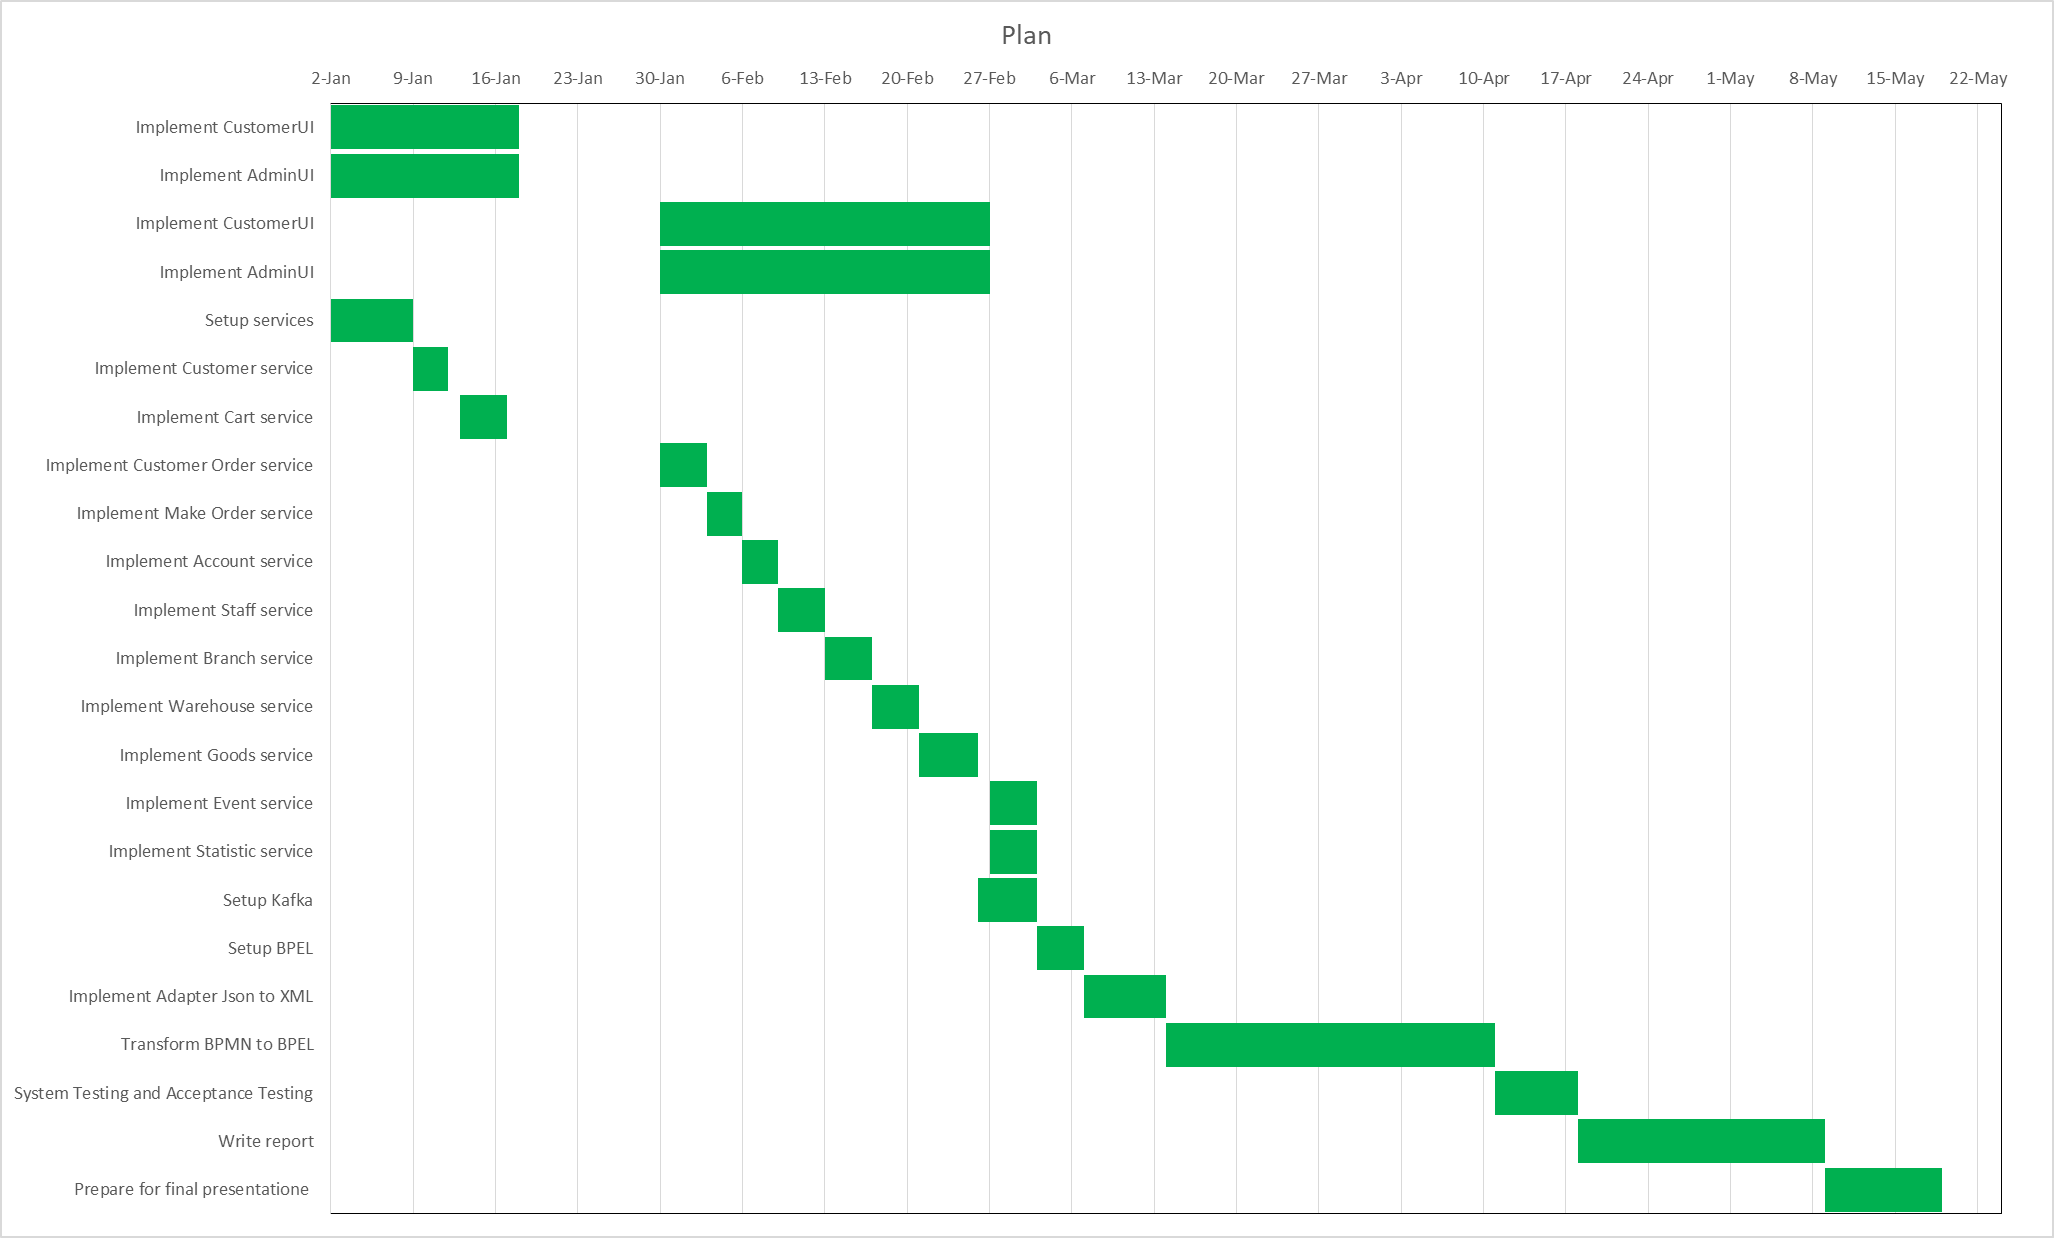
\includegraphics[width=14cm]{img/plan.png}
    \end{center}
    \caption{Biểu đồ Gantt cho kế hoạch đồ án tốt nghiệp}
\end{figure}

Lưu ý: Khoảng trống từ ngày 16/1 đến 29/1 là thời gian nghỉ tết

%%%%%%%%%%%%%%%%%%%%%%%%%
\subsection{Phân chia công việc}
